\documentclass[titlepage]{article}
\usepackage{graphicx} % Required for inserting images
\usepackage[backend=biber, style=ieee]{biblatex}
\addbibresource{references.bib}
\usepackage[
    top=3cm,
    bottom=3cm,
    left=2.5cm,
    right=2.5cm
]{geometry}
\usepackage{booktabs}
\usepackage{float}
\usepackage{amsmath}
\usepackage[hidelinks]{hyperref}
\usepackage{subcaption}
\usepackage{booktabs}
\usepackage{tabularx}
\usepackage{array}
\usepackage{ragged2e}
\usepackage{booktabs}

\title{
\Huge Big Data Analytics \\
\vspace{0.5em}
\Large Real-time Financial Transaction Anomaly Detection}

\author{
    Julia Kruk, Barbara Seweryn, Zuzanna Sieńko, Nadia Serafin \\
    \vspace{0.5em}
    \small Team: philodendron white measure \\
}

\date{October 2026}

\begin{document}
\maketitle

\tableofcontents

\newpage

\section{Project overview}
The objective of this project is to design and implement a real-time financial transaction monitoring and unsupervised anomaly detection system using Big Data technologies and machine learning.

The solution will follow a Lambda Architecture. It will combine three different data sources including batch processing of historical financial transactions and stream processing of incoming transaction events. Additionally, synthetically generated account activity data, including login events and device information, will be incorporated to provide more detailed context for anomaly detection. A data generation and ingestion component will publish transaction and account activity events to Apache Kafka, while the data will be stored in MinIO storage.

The batch layer will be responsible for training machine learning models on historical data and periodically retraining them as new data becomes available. In parallel, the speed layer will perform streaming inference by processing incoming transactions, applying the necessary preprocessing, and using latest trained model to generate anomaly risk prediction. Data processed in batch and speed layers will be available as real-time and batch views using Cassandra.

The results will be presented through an interactive dashboard using Streamlit. It will allow users to monitor transaction activity, investigate anomaly alerts and explore statistics related to user behaviour.

\section{Project deliverables from user's perspective}
From the user's perspective, the system will provide the following functionalities:
\begin{enumerate}
    \item Real-time transaction monitoring -- users will be able to observe incoming financial transactions and their anomaly risk prediction.
    \item Anomaly detection and alerts -- transactions identified as suspicious will be highlighted and presented in a dedicated alert section, drawing users' attention to those suspicious activities.
    \item Transaction investigation and statistics -- users will be able to examine individual transactions and explore overall transaction activity through interactive visualisations. The dashboard will present statistics such as transaction volumes, average transaction amounts, transaction type distributions, and transaction trends over time.
    \item Anomaly detection analytics and model performance -- users will be able to analyze the results of the anomaly detection system, including alert trends over time. The dashboard will also provide anomaly detection statistics, such as the number and percentage of detected anomalies, anomaly score distributions, and trends in detected anomalies over time.
\end{enumerate}


\section{Business process diagram for the core use-case}
\textbf{Business context}\\ 
The system is intended for the fraud team of a mobile money operator. The dominant fraud pattern in this setting is account takeover: an attacker gains access to a customer's account, transfers the balance to another account and cashes it out shortly afterwards. The operator's existing rule-based control catches only a small fraction of such cases, and the fraud team can review only a limited number of alerts per hour. The system therefore ranks incoming transactions by an anomaly score that combines the transaction itself, the account's recent login and device activity, and the history of the receiving account, so that analysts review the most suspicious transfers first and can freeze the destination account before the cash-out takes place.\\

\noindent \textbf{Actors}\\ 
The customer (account holder), the operator's core transaction system (executes transactions and emits events), the anomaly detection system (this project) and the fraud analyst (reviews alerts and decides).

\noindent \textbf{Process}\\
Figure~\ref{fig:bpmn_core} shows the process from the customer initiating a transaction to the recorded outcome. Transactions below the alert threshold complete without intervention. Alerts are reviewed by the analyst, who verifies with the customer and either freezes the accounts involved and blocks the pending cash-out, or releases the alert. Both decisions are recorded and feed the evaluation metrics on the dashboard.

\begin{figure}[H]
    \centering
    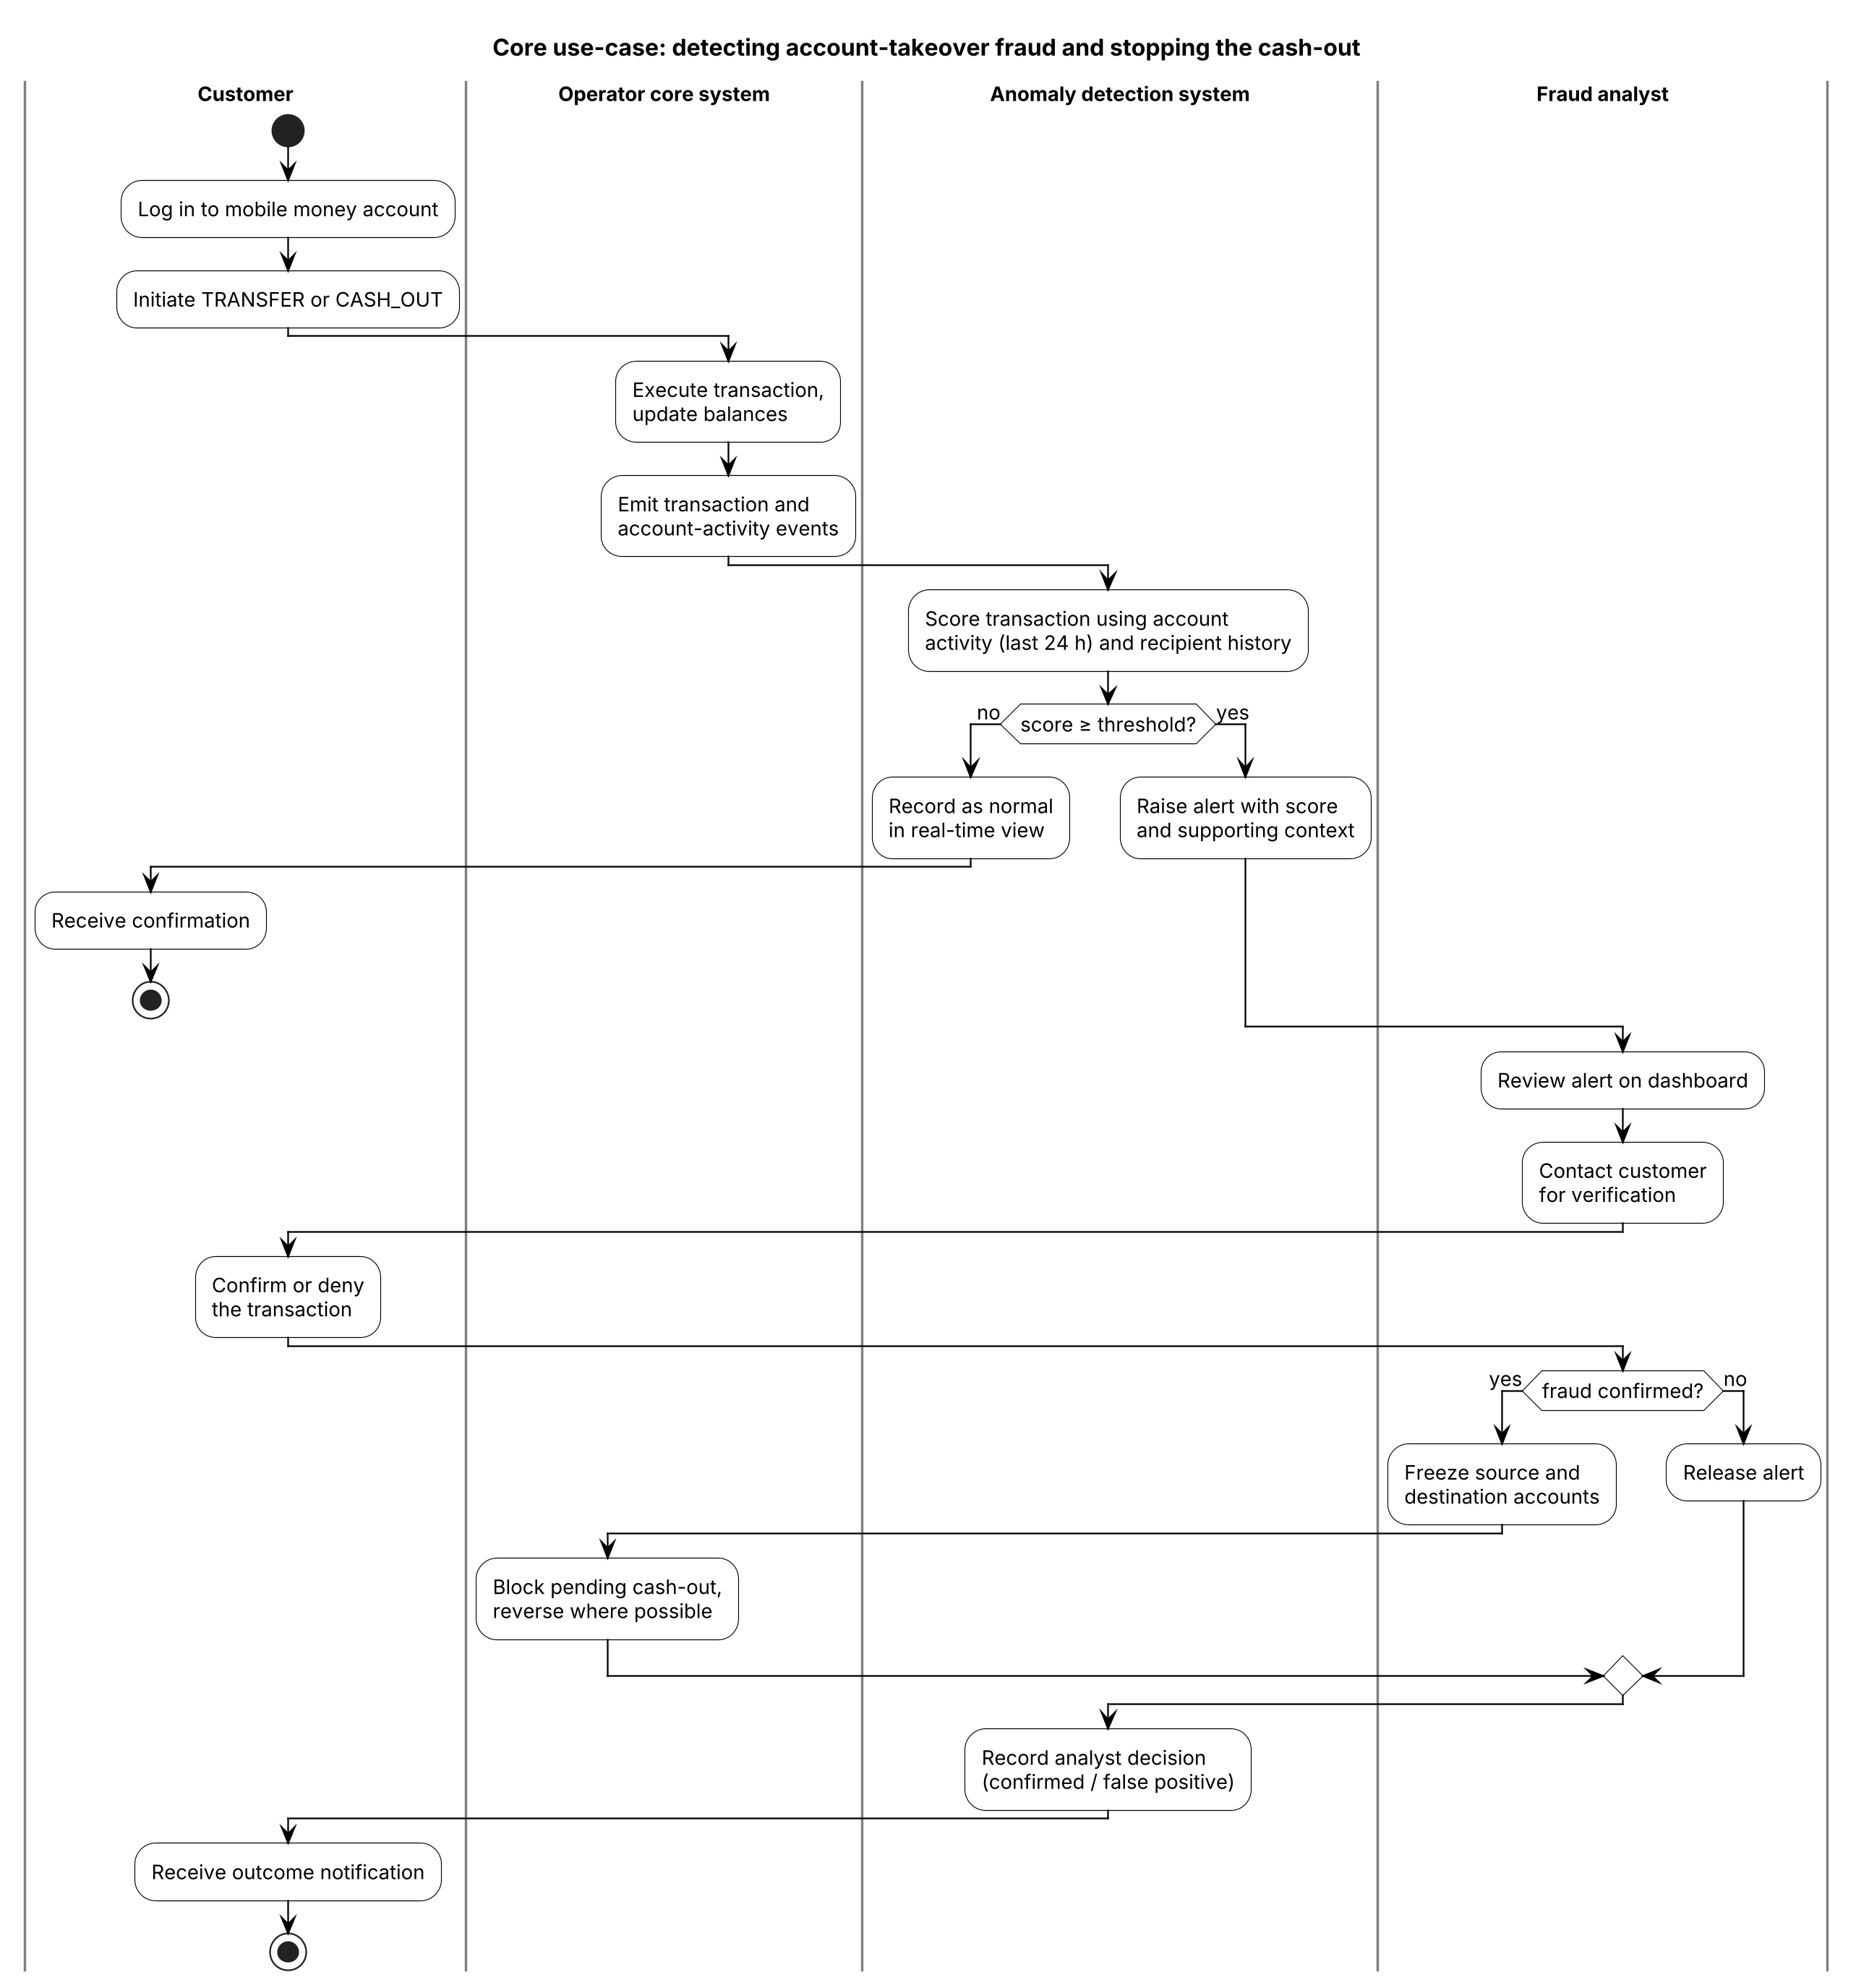
\includegraphics[width=0.95\textwidth]{report_plots/bpmn_core_use_case.png}
    \caption{Business process of the core use-case: detecting account-takeover fraud and stopping the cash-out}
    \label{fig:bpmn_core}
\end{figure}


\section{Data sources and their preliminary investigation}
\label{section:data_sources}
\subsection{PaySim -- financial transaction dataset}
PaySim is a synthetic dataset available on Kaggle: \href{https://www.kaggle.com/datasets/ealaxi/paysim1}{Synthetic Financial Datasets For Fraud Detection} simulating mobile money transactions, generated based on real transaction patterns from a financial service provider. It contains 6 362 620 records and 11 features. Those features and their types are shown in Table~\ref{tab:paysim_dtypes}.
\begin{table}[H]
    \centering
    \caption{Data types of the PaySim dataset attributes}
    \label{tab:paysim_dtypes}
    \begin{tabular}{ll}
        \toprule
        \textbf{Attribute} & \textbf{Data type} \\
        \midrule
        step & Integer \\
        type & String (categorical) \\
        amount & Float \\
        nameOrig & String \\
        oldbalanceOrg & Float \\
        newbalanceOrig & Float \\
        nameDest & String \\
        oldbalanceDest & Float \\
        newbalanceDest & Float \\
        isFraud & Integer \\
        isFlaggedFraud & Integer \\
        \bottomrule
    \end{tabular}
\end{table}
One simulation step represents one hour, with 743 observed steps spanning approximately 31 days.
The dataset contains two fraud-related fields: \texttt{isFraud} (identifying fraudulent transactions in the simulation) and \texttt{isFlaggedFraud} (representing an existing rule-based detection mechanism). Since the project focuses on unsupervised anomaly detection rather than supervised fraud classification, these labels will not be used as model input features or training targets. The objective is to identify transactions that deviate from typical patterns.

Preliminary exploratory data analysis revealed no missing values or duplicate records. The dataset contains five transaction types:
\begin{itemize}
    \item CASH\_OUT -- 35.17\% of all transactions,
    \item PAYMENT -- 33.81\% of all transactions,
    \item CASH\_IN -- 22.00\% of all transactions,
    \item TRANSFER -- 8.38\% of all transactions,
    \item DEBIT -- 0.65\% of all transactions.
\end{itemize}
Transaction amounts are right-skewed, with a median of approximately 74 872 and a mean of 179 862. The skewed distribution is visualized in Figure~\ref{fig:transaction_amounts}. Significant differences in transaction amounts between transaction types suggest that transaction type should be considered when identifying unusual patterns.
\begin{figure}[H]
    \centering
    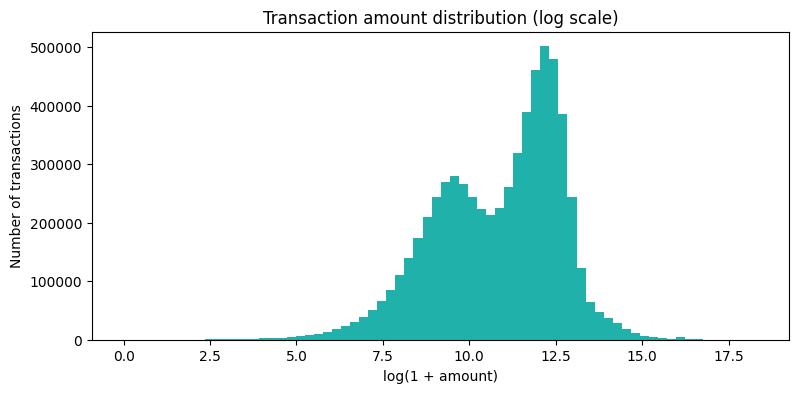
\includegraphics[width=0.8\textwidth]{report_plots/transaction_amount_dist.png}
    \caption{Distribution of transaction amounts (log scale)}
    \label{fig:transaction_amounts}
\end{figure}

Transaction activity varies over time, with hourly volumes ranging from 2 to 51 352 transactions. As it can be seen in Figure~\ref{fig:trans_vol_over_time}, there is a substantial decrease in transaction volume is observed after approximately step 400, indicating a significant change in transaction activity patterns. To ensure that the historical dataset includes observations from both periods, the data will be divided some time after step 400th, e.g. at step 500. Transactions from the first 500 simulation hours will be used as historical batch data, while the remaining transactions will be replayed as a simulated stream. The aim of this approach is to allow the model to learn from different transaction activity patterns.
\begin{figure}[H]
    \centering
    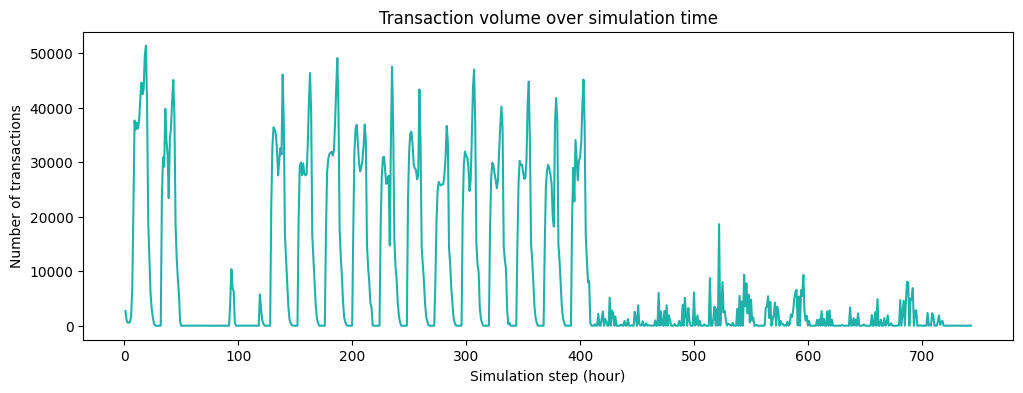
\includegraphics[width=0.8\textwidth]{report_plots/trans_volume_over_time.png}
    \caption{Transactions volume over time}
    \label{fig:trans_vol_over_time}
\end{figure}

The dataset contains 6 353 307 unique senders, indicating that nearly every sender appears only once. Only 814 streaming senders (0.27\%) also appear as senders in the historical dataset. Therefore, it is impossible to create individual sender profiles. Recipient identifiers show greater repetition, particularly for customer accounts (C), which receive an average of 7.36 transactions, compared with approximately one transaction per merchant (M). These findings are summarized in Table~\ref{tab:C_R_transactions}.
\begin{table}[H]
    \centering
    \caption{Customer and recipients transactions}
    \label{tab:C_R_transactions}
    \begin{tabular}{llll}
        \toprule
        \textbf{Recipient type} & \textbf{Transactions}  & \textbf{Unique recipients} & \textbf{Avg transactions per recipient}\\
        \midrule
        C & 4 211 125 & 571 961 & 7.36 \\
        M & 2 151 495 & 2 150 401 & 1.00 \\
        \bottomrule
    \end{tabular}
\end{table}
This suggests that historical recipient-level features may provide additional context, subject to their availability across the batch and streaming periods. Based on these findings, the proposed system will model typical transaction patterns rather than individual customer behaviour.

\subsection{Synthetic data generation}
\subsubsection{Reference dataset: IEEE-CIS Fraud Detection}
The IEEE-CIS Fraud Detection dataset is available on Kaggle: \href{https://www.kaggle.com/competitions/ieee-fraud-detection}{IEEE-CIS Fraud Detection}. It contains real-world e-commerce transaction records provided by Vesta Corporation. The dataset includes transaction-related features and partially anonymized identity information, such as device characteristics and browser details.

The analysis takes into consideration two files: the one related to transaction data, containing 590 540 transactions and 394 attributes, and the one associated with identity information, containing 144 233 records and 41 attributes. Identity records are available for only 24.42\% of transactions, meaning that the remaining 75.58\% have no corresponding records in the identity dataset. \\

\noindent \textbf{Data completeness and device characteristics}\\
Many IEEE-CIS attributes are anonymized. The preliminary analysis focuses on features whose interpretation can be inferred from their names and observed values. Selected attributes include \texttt{DeviceType}, \texttt{DeviceInfo}, \texttt{id\_30} (operating system), \texttt{id\_31} (browser), and \texttt{id\_33} (screen resolution). Additionally, \texttt{TransactionAmt}, \texttt{ProductCD}, and \texttt{isFraud} were included to examine relationships between device characteristics and transaction patterns. \texttt{TransactionID} was used to join the datasets, while \texttt{TransactionDT} provides relative reference transaction timing information.

Exploratory data analysis revealed varying levels of missing data among identity attributes. Within the identity dataset, \texttt{DeviceType} and browser information (\texttt{id\_31}) have relatively low missing-value rates of 2.37\% and 2.74\%, respectively. In contrast, operating system information (\texttt{id\_30}) is missing in 46.22\% of records, screen resolution (\texttt{id\_33}) in 49.19\%, and \texttt{DeviceInfo} in 17.73\%.

Among identity records, 59.05\% correspond to desktop devices and 38.58\% to mobile devices, while the remaining 2.37\% have an unknown device type. The most common device information values include Windows, iOS Device, and MacOS. Browser and operating system distributions also vary significantly between desktop and mobile devices. \\

\noindent \textbf{Device profile analysis}\\
To investigate dependencies between device attributes, combinations of device type, operating system, and browser were examined. The analysis identified 937 distinct device profiles, with the 20 most frequent combinations accounting for 51.51\% of identity records. These findings indicate that device attributes should not be generated independently. Instead, sampling complete profiles according to their observed frequencies can preserve realistic relationships between device characteristics.

Transactions associated with desktop devices have a higher mean amount (92.60) than those associated with mobile devices (69.50), with corresponding medians of 54.44 and 46.42. Product category distributions also differ by device type. For example, category C represents 52.42\% of mobile transactions compared with 37.39\% of desktop transactions. \\

\noindent \textbf{Transaction characteristics and fraud patterns}\\
The observed fraud rate is 6.52\% for desktop transactions and 10.17\% for mobile transactions. Furthermore, transactions with available identity records have a fraud rate of 7.85\%, compared with 2.09\% for transactions without identity records. These results show differences between groups of transactions, but it does not need to mean that device type or identity data availability causes a higher fraud risk.\\

\noindent \textbf{Impact for the generation of synthetic data}\\
The IEEE-CIS dataset will be used as a reference for generating synthetic device information that will complement PaySim transactions. Instead of directly copying IEEE-CIS records, the generator will use observed distributions and relationships between device attributes to create realistic device profiles.

The planned use of selected attributes is shown in Table~\ref{tab:ieee_attributes}.
\begin{table}[H]
    \centering
    \caption{IEEE-CIS attributes and their planned use in synthetic data generation}
    \label{tab:ieee_attributes}
    \small
    \renewcommand{\arraystretch}{1.3}
    \begin{tabularx}{\textwidth}{@{}lXX@{}}
        \toprule
        \textbf{IEEE-CIS attribute} & \textbf{Information provided} & \textbf{Planned use} \\
        \midrule

        \texttt{DeviceType} & Device type (mobile/desktop) & Generate device types, with proportions adjusted if necessary to better reflect PaySim's mobile money environment. \\

        \addlinespace

        \texttt{id\_30} & Operating system and version & Generate operating systems consistent with device types. \\

        \addlinespace

        \texttt{id\_31} & Browser and version & Generate browsers consistent with device types and operating systems. \\

        \addlinespace

        \texttt{DeviceInfo} & Device information, such as model or platform & Add further details to generated device profiles. \\

        \addlinespace

        \texttt{id\_33} & Screen resolution & Optionally include additional device characteristics. \\

        \addlinespace

        Combinations of device attributes & Observed relationships and frequencies & Generate coherent device profiles rather than sampling each attribute independently. \\

        \bottomrule
    \end{tabularx}
\end{table}

In addition to device profiles, we plan to introduce a separate synthetic account activity source, including events such as successful and failed logins and device changes. These events will not be generated entirely randomly, but will be partly influenced by the PaySim \texttt{isFraud} label to create more realistic account activity patterns.

\subsubsection{Planned synthetic data generation}
A synthetic account activity dataset will be generated to provide additional context for PaySim transactions. As mentioned above, the generated data will include structured events, such as successful and failed login attempts and device changes, together with account identifiers, timestamps, and device information. Device profiles will be based on distributions and relationships observed in the IEEE-CIS dataset, while account activity patterns will be generated using simulation assumptions and may be partly influenced by the PaySim isFraud label.
\begin{table}[H]
    \centering
    \caption{Proposed schema of synthetic data}
    \label{tab:synthetic_events_schema}
    \small
    \renewcommand{\arraystretch}{1.3}
    \begin{tabularx}{\textwidth}{@{}l l X@{}}
        \toprule
        \textbf{Attribute} & \textbf{Data type} & \textbf{Description} \\
        \midrule

        \texttt{event\_id} & String & Unique event identifier \\

        \addlinespace

        \texttt{account\_id} & String & Account identifier corresponding to \texttt{nameOrig} in PaySim \\

        \addlinespace

        \texttt{step} & Integer & Simulation hour corresponding to the PaySim timeline \\

        \addlinespace

        \texttt{event\_timestamp} & Datetime & Simulated event timestamp \\

        \addlinespace

        \texttt{event\_type} & String (categorical) & \texttt{LOGIN\_SUCCESS}, \texttt{LOGIN\_FAILED}, \texttt{DEVICE\_CHANGE} \\

        \addlinespace

        \texttt{device\_id} & String & Unique device identifier \\

        \addlinespace

        \texttt{device\_type} & String (categorical) & \texttt{mobile}, \texttt{desktop} \\

        \addlinespace

        \texttt{operating\_system} & String & Operating system and version \\

        \addlinespace

        \texttt{browser} & String & Browser and version \\

        \addlinespace

        \texttt{device\_info} & String & Additional device information \\

        \addlinespace

        \texttt{ip\_address} & String & Simulated IP address (optional) \\

        \addlinespace

        \texttt{country} & String & Simulated country (optional) \\

        \bottomrule
    \end{tabularx}
\end{table}

Since most sender accounts in PaySim appear only once, the dataset provides very limited information about individual user behaviour. To address this limitation, we plan to include in the synthetic dataset additional events and attributes for each account previously identified in the IEEE-CIS dataset. These events will represent account activity rather than financial transactions, which are already provided by PaySim.

The volume of synthetic data will depend on the number of PaySim accounts and the number of account activity events generated for each account. Synthetic account activity events and PaySim transactions will be sent to Apache Kafka to simulate real-time data processing. The rate at which events are sent will be configurable, allowing the system to be tested with different amounts of incoming data.

To make the stream realistic, the generator will inject controlled faults into the emitted events: missing attribute values, out-of-order delivery and duplicated events, each at a configurable rate. These faults are not corrected at the source; they are detected and resolved in the preprocessing step, as described in Section~\ref{sec:assumptions}.

Synthetic events will be divided into historical and streaming data using the same simulation timeline as PaySim.

\subsection{Reserve data source: IBM TabFormer credit card transactions}
\label{sec:tabformer}

The IBM TabFormer dataset is a synthetic credit card transaction dataset released by IBM together with the TabFormer
paper (Padhi et al., ICASSP 2021) and available on Kaggle: \href{https://www.kaggle.com/datasets/ealtman2019/credit-card-transactions}{Credit Card Transactions}
and on GitHub: \href{https://github.com/IBM/TabFormer}{IBM/TabFormer}. It contains approximately 24 million card transactions
generated for about 2\,000 synthetic users over a period of roughly three decades (1991--2020). Transactions are 
produced by a rule-based generator with stochastic sampling and include merchant, location and error information, 
together with a per-transaction fraud label (\texttt{Is Fraud?}, about 0.12\% of records). The attributes are
listed in Table~\ref{tab:tabformer}.

\begin{table}[H]
    \centering
    \caption{Attributes of the IBM TabFormer dataset}
    \label{tab:tabformer}
    \small
    \renewcommand{\arraystretch}{1.3}
    \begin{tabularx}{\textwidth}{@{}l l X@{}}
        \toprule
        \textbf{Attribute} & \textbf{Data type} & \textbf{Description} \\
        \midrule

        \texttt{User} & Integer & Synthetic user identifier \\

        \addlinespace

        \texttt{Card} & Integer & Card index within a user \\

        \addlinespace

        \texttt{Year}, \texttt{Month}, \texttt{Day} & Integer & Transaction date components \\

        \addlinespace

        \texttt{Time} & String (HH:MM) & Transaction time \\

        \addlinespace

        \texttt{Amount} & String & Amount with currency symbol; negative values represent refunds \\

        \addlinespace

        \texttt{Use Chip} & String (categorical) & \texttt{Swipe Transaction}, \texttt{Chip Transaction}, \texttt{Online Transaction} \\

        \addlinespace

        \texttt{Merchant Name} & Integer & Hashed merchant identifier \\

        \addlinespace

        \texttt{Merchant City} & String & Merchant city (\texttt{ONLINE} for online transactions) \\

        \addlinespace

        \texttt{Merchant State} & String & Merchant state or country; missing for online transactions \\

        \addlinespace

        \texttt{Zip} & Float & Merchant ZIP code; missing for online transactions \\

        \addlinespace

        \texttt{MCC} & Integer & Merchant category code \\

        \addlinespace

        \texttt{Errors?} & String & Comma-separated error flags, e.g.\ \texttt{Bad PIN}, \texttt{Insufficient Balance} \\

        \addlinespace

        \texttt{Is Fraud?} & String (categorical) & \texttt{Yes}, \texttt{No}; fraud label used for evaluation only \\

        \bottomrule
    \end{tabularx}
\end{table}

Compared with PaySim, this dataset provides a dense transaction history for every user (on average more than ten 
thousand transactions per user), a per-transaction label that matches transaction-level anomaly scoring, and a time 
span long enough to replay an effectively unbounded stream. These properties make it suitable for evaluating and 
tuning the anomaly detection model.\\

\noindent \textbf{Role in the project}\\
This dataset is treated as a \emph{reserve} data source. It will be used only if the primary sources (the PaySim transaction stream and the synthetic account activity events) turn out to be insufficient,  in particular if the volume of streaming data after the batch/stream split proves too small to evaluate and optimise the model in the later project phases. For this reason it is not described further in the following sections.

Should it be activated, it would be ingested as a second transaction source through the same Kafka, batch and speed layer components, after mapping its 
attributes to the common transaction schema used for PaySim, and its fraud label would be used exclusively for model
evaluation.

\section{Data processing and proposed infrastructure}
The data processing pipeline follows the Lambda Architecture principles, maintaining two parallel data flow paths: 
a \textbf{Batch Layer} for historical feature engineering and periodic ML model re-training, and a \textbf{Speed Layer} 
for low-latency streaming inference and real-time alert generation. The high-level data flow is shown in Figure~\ref{fig:architecture_diagram}; the assumptions in Section~\ref{sec:assumptions} refer to its elements by name.

\begin{figure}[H]
    \centering
    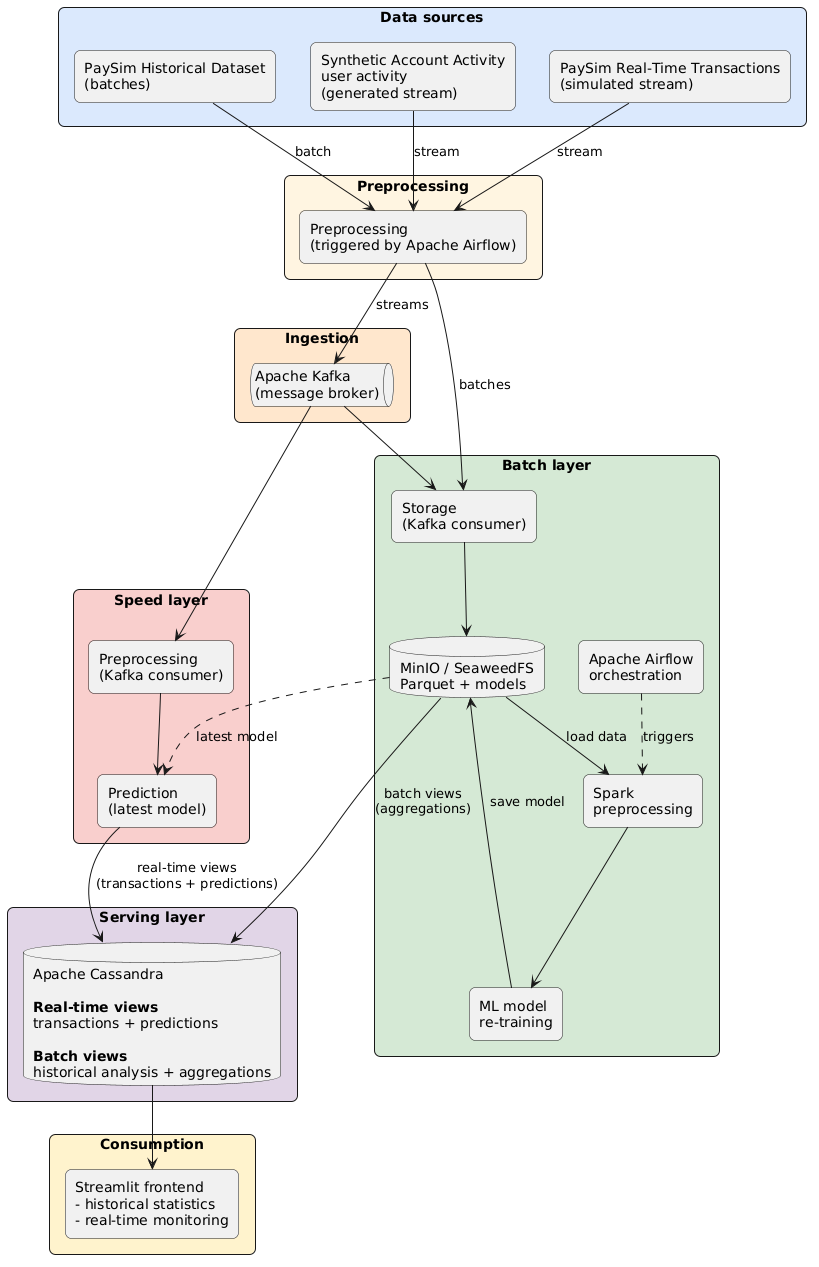
\includegraphics[width=0.8\textwidth]{report_plots/infrastructure_diagram.png}
    \caption{Data flow and solution architecture}
    \label{fig:architecture_diagram}
\end{figure}

\newpage
\subsection{Proposed infrastructure}
The proposed infrastructure consists of the following components:
\begin{itemize}
    \item Preprocessing -- In this component the first preprocessing of all data sources will be performed (checking data completeness, data cleansing, etc.).
    \item Ingestion layer -- Apache Kafka will serve as a message broker, routing the events to the next layers. The preprocessing component in the Speed layer and Storage component in the Batch layer will act as Kafka consumers.
    \item Batch layer -- Raw batch data will be stored in MinIO (or SeaweedFS) in Parquet format. Apache Airflow will orchestrate the process of retraining the machine learning model:
    \begin{itemize}
        \item Data will be loaded from the storage and preprocessed using Apache Spark;
        \item The ML model will be re-trained and saved back to the storage.
    \end{itemize}
    \item Speed layer -- The data will be preprocessed and the prediction will be generated using the latest model from the storage. This process will be handled by Apache Spark (or Kafka in Python). The data with the predictions will be sent to Serving layer.
    \item  Serving layer -- it will contain two types of views:
    \begin{itemize}
        \item Real-time views -- stored in Cassandra tables containing incoming transactions and their predictions;
        \item Batch views -- stored in Cassandra tables containing historical analysis and aggregations. 
        
    \end{itemize}
    \item Consumption -- The frontend part will be build using Streamlit. The user will be able to explore different views, such as real-time transaction monitoring or historical transaction statistics.
\end{itemize}


\subsection{Key assumptions regarding data processing}
\label{sec:assumptions}
Each assumption refers to an element of Figure~\ref{fig:architecture_diagram}.

\noindent \textbf{Sources and ingestion}
\begin{itemize}
    \item \textbf{Dataset splitting (Data sources).} PaySim transactions and synthetic account-activity events with \texttt{step} $\le 500$ form the historical batch data; later events are replayed as a stream. One step is one simulated hour in every layer.
    \item \textbf{Stream replay (Data sources $\rightarrow$ Ingestion).} Both streams are replayed along the same timeline, one step per $R$ seconds (initially $R = 10$, i.e.\ about 0.2--5\,100 events/s). One message carries one event; transactions and account activity use separate topics keyed by account identifier.
    \item \textbf{Stream perturbation (Data sources $\rightarrow$ Ingestion).} The generator injects faults into the emitted events: missing attribute values (initially 2\% of events), out-of-order events (1\%, delayed by up to two steps) and duplicates (0.5\%). Rates are configurable; faults are not corrected at the source.
    \item \textbf{Delivery (Ingestion).} Delivery is at-least-once. Each event carries its own event time (\texttt{step}, \texttt{event\_timestamp}), so arrival order is not assumed to match event order.
\end{itemize}

\noindent \textbf{Batch path}
\begin{itemize}
    \item \textbf{Storage (Storage $\rightarrow$ MinIO).} Raw events are appended, partitioned by \texttt{step} and event type; the store is append-only and is the system of record.
    \item \textbf{Preprocessing (Spark preprocessing).} One shared feature-engineering module is used by both layers, so training and inference see identical features. \texttt{isFraud} and \texttt{isFlaggedFraud} are never used as features or targets, only to compute dashboard evaluation metrics.
    \item \textbf{Fault handling (Spark preprocessing, Preprocessing).} Events missing a mandatory attribute are rejected and counted; missing optional attributes are set to \texttt{unknown}. Duplicates are collapsed by event identifier. Out-of-order events are re-sorted by event time in the batch path and flagged \texttt{late} in the speed path.
    \item \textbf{Model re-training (ML model re-training $\rightarrow$ MinIO).} An unsupervised model is re-trained every 24 steps on the full historical window and saved under a timestamped path with its threshold $\tau$ (99th percentile of training scores); the newest version is the \emph{latest model}.
    \item \textbf{Batch views (MinIO $\rightarrow$ Cassandra).} Aggregates and model metrics are fully recomputed after each re-training and overwritten.
\end{itemize}

\noindent \textbf{Speed path}
\begin{itemize}
    \item \textbf{Scoring (Preprocessing $\rightarrow$ Prediction).} Each event is scored statelessly from its own attributes and precomputed recipient-level aggregates from the batch views.
    \item \textbf{Model refresh (MinIO $\rightarrow$ Prediction).} The Speed Layer checks for a newer model every minute and swaps atomically; in-flight events keep the previous version.
    \item \textbf{Output (Prediction $\rightarrow$ Cassandra).} Each scored event carries its score and \texttt{is\_anomaly} $=$ (score $\ge \tau$); target latency Kafka $\rightarrow$ Cassandra below 2~s.
\end{itemize}

\noindent \textbf{Serving (Cassandra $\rightarrow$ Streamlit).} The dashboard reads only from Cassandra; real-time views are partitioned by \texttt{step}. All timestamps are simulated; wall-clock time only paces the replay.


\section{Preliminary allocation of tasks and responsibilities}

\renewcommand{\arraystretch}{1.4}
\setlength{\tabcolsep}{5pt}

\begin{table}[H]
\centering
\caption{Team responsibilities across project milestones}
\label{tab:team_responsibilities}

\footnotesize

\begin{tabularx}{\linewidth}{|>{\RaggedRight\arraybackslash}p{2cm}|*{4}{>{\RaggedRight\arraybackslash}X|}}
\toprule

\textbf{\mbox{Team} \mbox{Member}}
    & \textbf{M1} & \textbf{M2} & \textbf{M3} & \textbf{M4} \\
    \toprule

    \textbf{Julia Kruk}
    & Defining system infrastructure, investigation of the technologies.
    & System containerization via Docker, streaming real-time transaction data to Apache Kafka, and implementing low-latency preprocessing (handling out-of-order events and missing values).
    & Integrating streaming preprocessing with the analytical module and optimizing processing latency.
    & Finalizing containerization, deployment configuration, and end-to-end integration testing. \\
    \midrule

    \textbf{\mbox{Nadia} \mbox{Serafin}}
    & Investigating data sources, defining synthetic data assumptions, defining user functionalities.
    & Generating synthetic account activity data and building historical data pipelines with Apache Spark.
    & Developing and evaluating anomaly detection models, performing EDA, and selecting evaluation metrics.
    & Optimizing anomaly detection models and evaluating final analytical results. \\
    \midrule

    \textbf{Barbara Seweryn}
    & Defining data storage requirements, historical data partitioning, and batch processing assumptions.
    & Managing MinIO storage, implementing historical data ingestion, and simulating real-world stream disturbances.
    & Configuring Apache Airflow for automated model re-training and integrating batch processing with the analytical module.
    & Finalizing automated workflows, validating pipeline reliability, and performing end-to-end testing. \\
    \midrule

    \textbf{Zuzanna Sieńko}
    & Defining business context and business process diagram. Investigating reserve data source.
    & Designing Apache Cassandra tables (Real-Time and Batch Views) and preparing data storage for analytical results.
    & Executing real-time ML inference and developing the Streamlit dashboard.
    & Finalizing the dashboard, anomaly alerts, and visualizations, and evaluating the solution from a business perspective. \\
    \bottomrule

\end{tabularx}
\end{table}


\section{Updates to PM1 Report}

The updates to the PM1 report include the following changes:
\begin{itemize}
    \item Instead of using the official MinIO server, we decided to use the pgsty/silo substitute. It is fully compatible with API S3 interface, while also deploying faster and being more lightweight. This change was made, because of problem with MinIO public pull policy for free accounts, which blocked fetching of MinIO latest image from Docker Hub. 
    \item We generated successful and failed login events using device information from IEEE-CIS. Four login scenarios and two activity patterns were added. The generated data was saved in Parquet format.
    \item We added \texttt{second\_offset} and \texttt{event\_time} to place transactions and login events on the same timeline.
    \item PaySim was split into historical and streaming data. The data was saved in Parquet format, and Apache Spark was used to check, transform, and summarize historical transactions.
\end{itemize}


\section{Conceptual Data Model}
The system combines financial transactions from PaySim with synthetically generated account activity events and device information. Although the data is organised into three parts: historical transactions, streaming transactions, and login events, in the conceptual data model one can distinguish four main entities: Account, Transaction, Login Event, and Device. 

Historical and streaming transactions represent the same entity, \textit{Transaction}, as they share a common structure and differ only in their role within the processing architecture. Each transaction involves a source and a destination \textit{Account}. \textit{Login Events} are associated with accounts through the \texttt{account\_id} attribute, which corresponds to \texttt{nameOrig} in PaySim. Each login event also contains a device identifier and its characteristics, represented conceptually by the \textit{Device} entity.

The relationships between these entities is shown in Figure~\ref{fig:conceptual_data_model}

\begin{figure}[H]
    \centering
    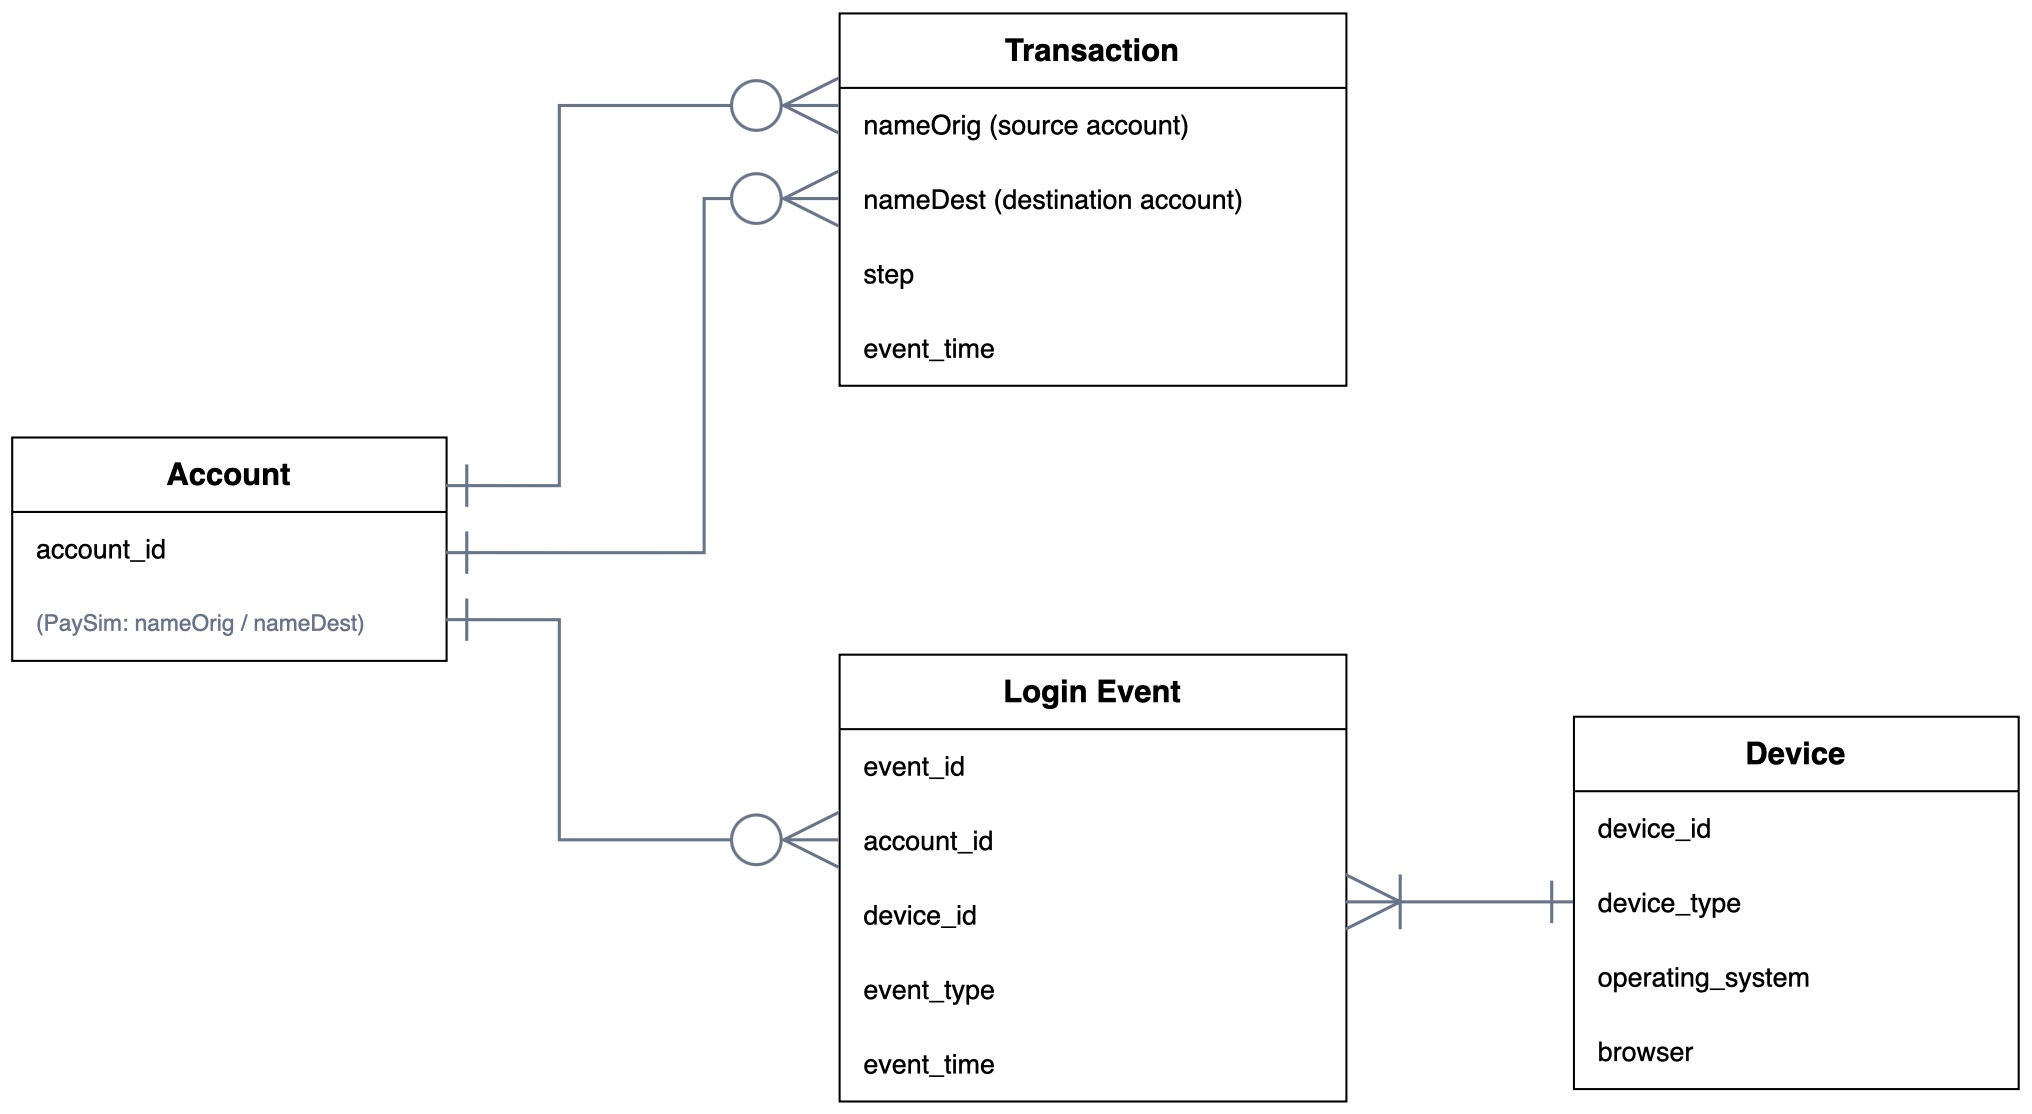
\includegraphics[width=0.8\textwidth]{report_plots/conceptual_data_model.png}
    \caption{Conceptual data model of financial transactions, accounts, login events, and devices.}
    \label{fig:conceptual_data_model}
\end{figure}


\section{Description of Data Sets}
\label{section:data_sets_description}
The PaySim dataset is used as the primary source of transaction data, while the IEEE-CIS dataset serves as a reference for generating synthetic device information. The IBM TabFormer dataset is reserved for potential use if the primary sources prove insufficient.
\subsection{PaySim Transaction Data}
The dataset was described in Section~\ref{section:data_sources}. The dataset was extended with two additional temporal attributes, \texttt{second\_offset} and \texttt{event\_time} and divided into historical (steps 1-500) and streaming (steps 501-743) subsets. Both subsets were saved in Parquet format for further processing.

The prepared PaySim datasets contain the original 11 PaySim attributes and two additional temporal attributes, as presented in Table~\ref{tab:paysim_data_description}.

The additional temporal attributes provide a common time representation for financial transactions and synthetically generated login events. The \texttt{second\_offset} attribute was set to zero for all PaySim transactions, as the original dataset provides only hourly time steps. The \texttt{event\_time} attribute was calculated as $(\text{step} - 1) \times 3600$, representing the transaction time in seconds relative to the beginning of the simulation. These attributes allow login events to be assigned more precise timestamps, "inside" the hours (steps), while maintaining temporal consistency with PaySim transactions.

The original \texttt{isFraud} and \texttt{isFlaggedFraud} attributes were kept in the prepared datasets. However, they are not intended to be used as input features for the unsupervised anomaly detection models. Instead, they will be used for evaluating the detection results against the available fraud-related labels.

\begin{table}[H]
    \centering
    \caption{Attributes of the prepared PaySim transaction datasets.}
    \label{tab:paysim_data_description}
    \small
    \begin{tabular}{lll}
        \toprule
        \textbf{Attribute} & \textbf{Data type} & \textbf{Description}\\
        \midrule
        step & Integer & Simulation time step, where each step represents one hour.\\
        type & String (categorical) & Transaction type: CASH\_IN, CASH\_OUT, DEBIT, PAYMENT, TRANSFER.\\
        amount & Float & Transaction amount.\\
        nameOrig & String & Identifier of the source account. \\
        oldbalanceOrg & Float & Source account balance before the transaction.\\
        newbalanceOrig & Float & Source account balance after the transaction. \\
        nameDest & String & Identifier of the destination account. \\
        oldbalanceDest & Float & Destination account balance before the transaction.\\
        newbalanceDest & Float & Destination account balance after the transaction. \\
        isFraud & Integer & Binary label indicating whether the transaction is fraudulent. \\
        isFlaggedFraud & Integer & Binary indicator of transactions flagged by PaySim's built-in detection rule. \\
        second\_offset & Integer & Number of seconds that have passed within a given simulation step. \\
        event\_time & Integer &Nnumber of seconds that have passed since the simulation began. \\
        \bottomrule
    \end{tabular}
\end{table}

\subsection{Synthetic Login Events}
\subsubsection{Synthetic Login Events - description}
As stated in Section~\ref{section:data_sources}, synthetic account activity data was introduced to enrich PaySim transactions with additional information about user behavior and devices.

Synthetic login events were generated exclusively for the streaming period (steps 501–743). Each event contains an account identifier, an event type, a device identifier, device characteristics, and temporal attributes. The dataset was saved in Parquet format. The attributes are presented below in Table~\ref{tab:login_data_description}.

\begin{table}[H]
    \centering
    \caption{Attributes of the synthetic login event dataset.}
    \label{tab:login_data_description}
    \small
    \begin{tabular}{lll}
        \toprule
        \textbf{Attribute} & \textbf{Data type} & \textbf{Description}\\
        \midrule
        event\_id & String & Unique identifier of the generated login event.\\
        account\_id & String & Identifier of the associated PaySim source account (nameOrig).\\
        device\_id & String & Identifier of the device assigned to the account.\\
        event\_type & String (categorical) & Login event type: LOGIN\_SUCCESS or LOGIN\_FAILED.\\
        step & Integer & PaySim simulation step corresponding to the event.\\
        second\_offset & Integer & Number of seconds elapsed within the simulation step.\\
        event\_time & Integer & Number of seconds elapsed since the beginning of the simulation.\\
        device\_type & String (categorical) & Device category, such as desktop or mobile.\\
        operating\_system & String & Operating system associated with the device.\\
        browser & String & Browser associated with the device.\\
        device\_info & String & Additional device information obtained from IEEE-CIS.\\
        screen\_resolution & String & Screen resolution associated with the device.\\
        \bottomrule
    \end{tabular}
\end{table}

Login events are assigned timestamps with second-level precision, allowing multiple events to occur within a single simulation step and enabling their chronological ordering relative to financial transactions. Each account with generated login activity is assigned a single device identifier and a consistent set of device characteristics. The dataset contains only complete device profiles selected from IEEE-CIS, avoiding missing values in the five device attributes used for generation. The generated records are also linked to existing PaySim source accounts through \texttt{account\_id}.

\subsubsection{Synthetic Login Events -- generation process}
The generation process consisted of the following steps:
\begin{enumerate}
    \item Account selection -- all accounts from the streaming transaction PaySim dataset were selected for synthetic login event generation. The implementation also supports selecting a smaller sample of accounts for testing purposes. For each selected account, the first transaction step is determined to ensure that login events were generated before the associated transaction.
    \item Device profile selection and assignment -- five device attributes were selected from the IEEE-CIS identity dataset: \texttt{DeviceType} (device category), \texttt{id\_30} (operating system), \texttt{id\_31} (browser), \texttt{DeviceInfo} (additional device information), and \texttt{id\_33} (screen resolution).\\
    Records containing missing values in any of these attributes were excluded. Unique complete device profiles were identified along with their frequencies, computed as the number of identity records in which each profile appears.\\
    To preserve the original proportions of device types, which may be distorted by the exclusion of incomplete records, profiles were sampled based on two factors: the frequency of each device type in the original dataset and the frequency of each complete profile within that device type:
    \[
        P(p_i) = P(d_i) \cdot P(p_i \mid d_i)
    \]
    where $P(p_i)$ is the sampling probability of device profile $p_i$, $P(d_i)$ is the proportion of device type $d_i$ in the original dataset (excluding records with unknown device types), and $P(p_i \mid d_i)$ is the relative frequency of profile $p_i$ among complete profiles of that device type.\\
    The resulting weights were normalized to sum to one. Each selected account was then assigned one sampled device profile and a unique \texttt{device\_id}.
    \item Login scenario and activity pattern assignment -- each account was randomly assigned one of four login scenarios: NORMAL\_LOGIN (65\%), SINGLE\_FAILURE (20\%), MULTIPLE\_FAILURES (5\%), or MULTIPLE\_LOGINS (10\%). Additionally, one of two activity patterns was assigned: SHORT\_ACTIVITY (70\%) or MIXED\_ACTIVITY (30\%). The login scenario determined the sequence of successful and failed login attempts, while the activity pattern determined their temporal distribution.
    \item Login event generation -- login sequences were generated before each account's first streaming transaction. For SHORT\_ACTIVITY, events were placed within the preceding six hours. For MIXED\_ACTIVITY, events were usually generated within the same six-hour window (80\% probability), but could also occur earlier in the streaming period (20\% probability). Accounts whose first transaction occurred in the first streaming step were excluded from event generation.
    \item Timestamp calculation -- each generated login event received an \texttt{event\_time} value representing seconds passed since the beginning of the simulation. The corresponding \texttt{step} and \texttt{second\_offset} were calculated from this timestamp. To maintain consistency with the prepared transaction data, where all transactions were assigned to the beginning of their simulation steps (\texttt{second\_offset} = 0), login events were assigned timestamps with second-level precision, ensuring that they occurred before each account's first transaction.
\end{enumerate}

\section{Data Acquisition and Transformation}
\subsection{Data Acquisition and Preparation}
Data acquisition and preparation were implemented in Python using Pandas and NumPy. The PaySim and IEEE-CIS datasets were loaded from CSV files and prepared as described in Section~\ref{section:data_sets_description}. The resulting datasets were saved in Parquet format: \texttt{paysim\_batch.parquet} for historical processing, and \texttt{paysim\_stream.parquet} and \texttt{login\_events.parquet} for streaming simulation. Parquet was selected as a columnar storage format suitable for efficient data processing with Apache Spark.

\subsection{Streaming Data Simulation and Kafka Ingestion}\label{sec:stream-sim}
The simulation of streams was implemented in \texttt{StreamProducer} class. The data from \texttt{paysim\_stream.parquet} and \texttt{login\_events.parquet} files is loaded and processed:
\begin{enumerate}
    \item Files are devided into streams based on the value in column `step' (each unique `step' value is a next stream).
    \item Paysim data is corrupted:
    \begin{itemize}
        \item with probability $p = 2\%$ value in randomely selected column is removed;
        \item with probability $p = 0.5\%$ row is duplicated;
        \item with probability $p = 1\%$ row is delayed and sent in the next stream;
    \end{itemize}
    \item Streams are produced to Kafka \texttt{raw-transactions} and \texttt{raw-logins} topics every 10 seconds .
\end{enumerate}

\subsection{Historical Data Processing with Apache Spark}\label{sec:historical}
A historical data processing pipeline was implemented using PySpark to validate, transform, and aggregate transaction data. The pipeline consists of the following stages:
\begin{enumerate}
    \item Data loading -- historical transaction data is loaded from MinIO in Parquet format using Apache Spark and the S3A connector.
    \item Data validation -- the pipeline checks the presence of required columns and identifies missing values, negative transaction amounts, invalid transaction types, and simulation steps outside the historical data range (1–-500). Validation results are logged for inspection.
    \item Feature engineering -- six additional features are calculated to provide information about transaction amounts, account balances, and temporal patterns:
    \begin{table}[H]
    \centering
    \caption{Features generated during historical data processing.}
    \label{tab:historical_features}
    \small
    \begin{tabular}{lp{9cm}}
        \toprule
        \textbf{Feature} & \textbf{Description}\\
        \midrule
        amount\_log & Logarithmic transformation of the transaction amount using log1p.\\
        hour\_of\_day & Hour of the day derived from the simulation step (0--23).\\
        day & Simulation day derived from the transaction step.\\
        orig\_balance\_diff & Difference between the source account balance before and after the transaction.\\
        dest\_balance\_diff & Difference between the destination account balance after and before the transaction.\\
        amount\_to\_balance\_ratio & Ratio of the transaction amount to the initial source account balance, calculated only when the balance is positive.\\
        \bottomrule
    \end{tabular}
    \end{table}

    \item Data aggregation -- three aggregated datasets were created to summarize transaction activity and provide statistics for the dashboard further in the project.
    \begin{table}[H]
        \centering
        \caption{Aggregations generated during historical data processing.}\label{tab:historical_aggregations}
        \small
        \begin{tabular}{lp{9cm}}
            \toprule
            \textbf{Aggregation} & \textbf{Description}\\
            \midrule
            Hourly statistics & Transaction count, total amount, average amount, approximate median amount, and maximum amount for each simulation step.\\
            Hourly statistics by type & Transaction count, total amount, and average amount grouped by simulation step and transaction type.\\
            Statistics by type & Transaction count, total amount, and average amount grouped by transaction type.\\
            \bottomrule
        \end{tabular}
    \end{table}

    \item Data storage -- the enhanced transaction dataset and the three aggregated datasets were saved to MinIO in Parquet format for further processing and analysis.

\end{enumerate}

\subsection{Data Storage}

To satisfy the requirements of the Lambda Architecture, the batch layer stores historical data in MinIO-like storage - \texttt{pgsty/silo} (\url{https://github.com/pgsty/silo}), an S3-compatible object storage server deployed directly inside the local Docker environment.
Because \texttt{pgsty/silo} maintains compatibility with Amazon S3 and the MinIO ecosystem, standard client libraries such as Python's \texttt{boto3} interact with the storage layer without requiring custom adapters or modified code.
In addition, \texttt{pgsty/silo} is lightweight and deploys quickly and has a web dashboard.
The storage container is defined in the \texttt{docker-compose.yaml} file as \texttt{'minio'}. 

The storage bucket structure is initialized upon startup in the \texttt{run\_minio.py} script. The script connects to the storage endpoint using root credentials, and ensures that required buckets exist before data ingestion or processing commences. If a bucket does not exist, it is created. The bucket structure is as follows:
\begin{itemize}
    \item \texttt{historical-data} bucket: Stores the historical PaySim dataset (steps 1--500), which is uploaded during initial setup and serves as the core data source for batch historical processing.
    \item \texttt{raw-transactions-data} bucket: Stores transaction data streams in Parquet format, processed using PySpark, partitioned by step and event type.
    \item \texttt{raw-logins-data} bucket: Stores login data streams in Parquet format, processed using PySpark, partitioned by step.
    % \item \texttt{clean-transactions-data} bucket: Contains cleaned, deduplicated, and validated streaming transactions. Populated by the stream consumer pipeline from Kafka messages, which cleans incoming transactions and stores them in the bucket.
    % \item \texttt{clean-logins-data} bucket: Analogous to the \texttt{clean-transactions-data} bucket, this bucket stores cleaned streaming login events. The stream consumer pipeline processes incoming login events from Kafka, performs validation and cleaning, and saves them in this bucket.
    \item \texttt{processed-data} bucket: Will contain the processed datasets generated by the batch processing pipeline. This bucket is used for storing the enhanced historical dataset and aggregated statistics, which are later used for model training and dashboard visualizations. This pipeline has not yet been included in Apache Airflow, but will be integrated in the next project phase.
\end{itemize}

\subsection{Serving Layer -- Apache Cassandra}\label{sec:cassandra}

The serving layer keeps the real-time and batch views will be read by the Streamlit dashboard in Apache Cassandra 5.0, run as a single-node service in \texttt{docker-compose.yaml}. 
The schema (\texttt{serving\_layer/schema.cql}, keyspace \texttt{fraud\_detection}) is applied automatically at start-up.
The tables were designed query-first: each table serves one dashboard query, the partition key is the attribute the dashboard filters on, and the clustering key gives the order in which rows are read.

Real-time views are partitioned by \texttt{step}, so a dashboard refresh reads one partition of at most a few thousand rows; batch views are partitioned by simulation \texttt{day} or by recipient. 
Table~\ref{tab:cassandra_tables} lists the seven tables.

\begin{table}[H]
    \centering
    \caption{Cassandra tables of the serving layer.}
    \label{tab:cassandra_tables}
    \small
    \renewcommand{\arraystretch}{1.3}
    \begin{tabularx}{\textwidth}{@{}l l >{\RaggedRight\arraybackslash}p{3.8cm} X@{}}
        \toprule
        \textbf{Table} & \textbf{View} & \textbf{Primary key} & \textbf{Content and dashboard use} \\
        \midrule
        \texttt{transactions\_by\_step} & real-time & (\texttt{step}), \texttt{event\_time} $\downarrow$, \texttt{tx\_id} & Every scored streaming transaction with its PaySim attributes, \texttt{anomaly\_score}, \texttt{is\_anomaly}, \texttt{model\_version} and \texttt{is\_late}. Live transaction monitor. \\
        \addlinespace
        \texttt{alerts\_by\_step} & real-time & (\texttt{step}), \texttt{anomaly\_score} $\downarrow$, \texttt{tx\_id} & Transactions above the threshold, highest score first, with analyst decision fields (\texttt{status}, \texttt{decided\_at}, \texttt{decided\_by}). Alert queue. \\
        \addlinespace
        \texttt{login\_events\_by\_account} & real-time & (\texttt{account\_id}), \texttt{event\_time} $\downarrow$, \texttt{event\_id} & Login events with device profile, newest first per account. Context panel when an alert is investigated. \\
        \addlinespace
        \texttt{transaction\_stats\_by\_step} & batch & (\texttt{day}), \texttt{step} & Per-step count, total, average and maximum amount, plus per-type maps. Historical volume and amount charts. \\
        \addlinespace
        \texttt{recipient\_profiles} & batch & (\texttt{name\_dest}) & Aggregates per destination account (count, amounts, distinct senders, cash-out and transfer counts). Lookup of the receiving account's history during scoring and investigation. \\
        \addlinespace
        \texttt{model\_runs} & analytical & (\texttt{model\_name}), \texttt{trained\_at} $\downarrow$ & One row per re-training: training window, threshold $\tau$, metrics map, artifact path. Model history; the first row is the latest model. \\
        \addlinespace
        \texttt{anomaly\_stats\_by\_step} & analytical & (\texttt{day}), \texttt{step} & Per-step number of scored events and anomalies, anomaly rate, score percentiles and precision/recall against the PaySim labels. Detection-statistics charts. \\
        \bottomrule
    \end{tabularx}
\end{table}

Two design choices follow from the PM1 assumptions. First, real-time rows are never updated: a transaction is written once with its score, and an analyst decision is written to \texttt{alerts\_by\_step} only. 
Second, batch views are overwritten after each re-training (Section~\ref{sec:assumptions}).

The schema was verified on the running stack: the seven tables are created by \texttt{cassandra-init}, and a round-trip test (insert into \texttt{transactions\_by\_step} and \texttt{alerts\_by\_step}, read back by \texttt{step}) returned the inserted rows.
Loading the views with data -- the scored stream from the speed layer and the Spark aggregates from the batch layer -- is part of Milestone 3, as both producers are completed in that phase.


\section{System Architecture}
\subsection{Diagram, description and data flows}
Figure \ref{fig:archm2} shows updated system architecture. The description of data flows is limited to the part of the system that is already implemented.
\subsection{Containerization with Docker}
The system is contenerized using Docker. Docker images are used to run Apache Kafka, Silo, Apache Cassandra, Apache Airflow, Postgres (for Apache Airflow), and Apache Spark. After running \texttt{docker compose up} the system starts to run -- Silo buckets and Cassandra tables are created, Kafka starts working.
\subsection{Stream data flow}

Transactions and login data are sent as messages to two topics in Kafka (\texttt{raw-transactions} and \texttt{raw-logins}). Kafka consumer is triggered by Apache Airflow -- every 60 seconds a DAG is run to consume latest messages and save them to buckets (\texttt{raw-transactions-data}, \texttt{raw-logins-data}) partitioned by step (both sources) and event type (transactions) in Silo.
\subsection{Historical data}
PaySim historical data are saved to Silo bucket imediately after starting the Docker containers. Then, they are processed using Apache Spark as described in Section~\ref{sec:historical}.
\begin{figure}[H]
    \centering
    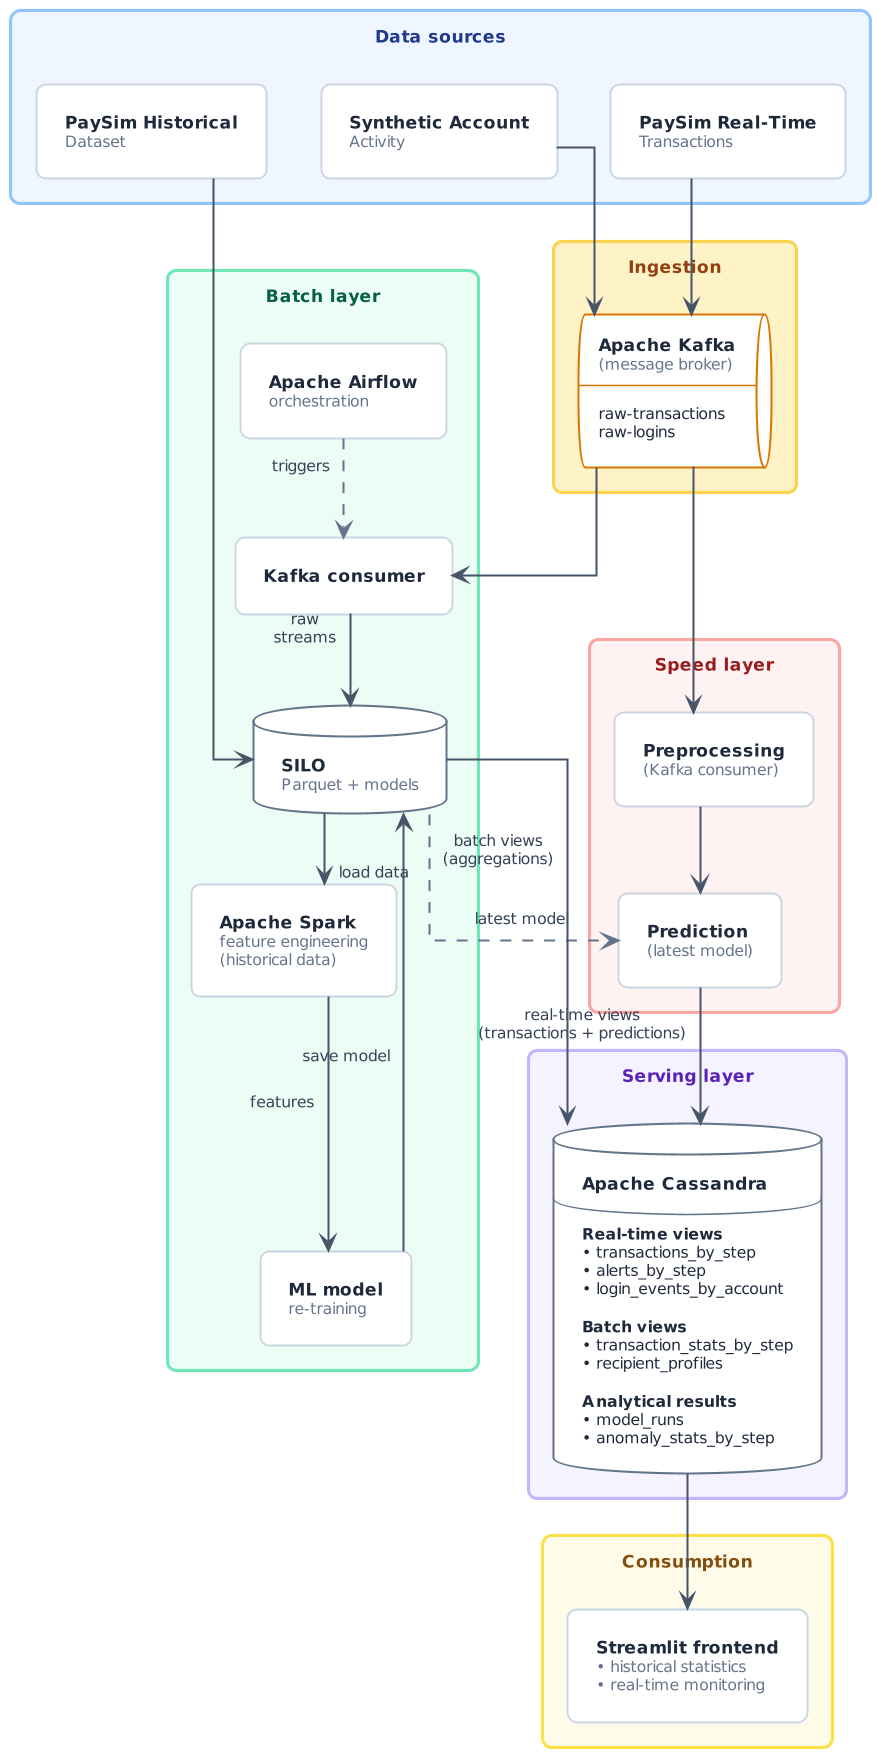
\includegraphics[width=0.65\textwidth]{report_plots/arch-updated.png}
    \caption{Updated system architecture}
    \label{fig:archm2}
\end{figure}

\subsection{Technologies and tools}
Currently used tools include:
\begin{itemize}
    \item Docker -- every external tool is used via its Docker image;
    \item Apache Kafka -- producer and consumer are implemented as fields in classes \texttt{StreamProducer} and \texttt{StreamConsumer}, the former class produces messages (streams) to two topics, the latter consumes cleaned streams;
    \item Silo -- historical data and cleaned stream data are stored in Silo buckets;
    \item Apache Airflow -- orchestrates uploading cleaned streams to Silo;
    \item Apache Cassandra -- 
    \item Apache Spark -- used for feature engineering applied to historical data 
\end{itemize}
\subsection{Data flows}


\section{Analytical Approach}
In the final dashboard user will be able to monitor real-time transaction activity, review historical statistics, and investigate the incoming transactions that has been labeled as suspicious by the anomaly detection model. 

To detect suspicious transactions, we will use an unsupervised anomaly detection model. The model will be trained on historical data and when a new batch of data is received, it will be retrained incrementally. This way the model will adapt to possible changes in the data distribution, i.e concept drift. The new, retrained model will then replace the previous model, and the predictions for the new transactions will be generated using the latest model. 
To avoid prediction latency during the training of the new model, a shadow model approach will be used (the previous model will still be used to generate predictions for incoming transactions and only when the re-training is completed, the new model will replace the previous one).
When a new transaction is processed, the model will assign an anomaly score to it based on how much it deviates from the learned patterns. If the score exceeds a predefined threshold, the transaction will be flagged as suspicious and an alert will be generated for further investigation. 

Following this approach, the batch layer will be responsible for training the model on historical data and re-training the model periodically on new batches of data. The re-training will be automated and triggered by Apache Airflow.
In the speed layer predictions for incoming transactions will be made and suspicious transactions will be flagged. 

\section{Planned use of GenAI}
GenAI tools will be used as a supportive assistance. Specifically, it will be used for:
\begin{itemize}
    \item help with research;
    \item code assistance to explore implementation alternatives;
    \item styling the dashboard (e.g., CSS);
    \item debugging potential errors;
    \item grammar improvement of the report, creating LaTex tables and diagrams.
\end{itemize}

Links to LLM conversations:
\begin{itemize}
    \item \href{https://chatgpt.com/share/6af975cb-3cb0-83eb-9d00-6415159ec66b}{Conversation 1}
    \item \href{https://chatgpt.com/share/6b030060-cb88-83ed-bb4f-f7726704a61b}{Conversation 2}
    \item \href{https://share.gemini.google/Gyx7zNGD21rM}{Conversation 3}
    \item \href{https://claude.ai/share/58832e26-37f8-44c1-944e-3b1c76014795}{Conversation 4}
\end{itemize} 

\newpage
% ----------------------------  LIST OF FIGURES --------------------------------
\listoffigures
\thispagestyle{empty}

% -----------------------------  LIST OF TABLES --------------------------------
\renewcommand{\listtablename}{List of tables}
\listoftables
\thispagestyle{empty}

\end{document}